% !TEX root = ../../phdthesis_tawatr.tex 

%% ==== ==== ==== ==== 
		
\section[Berdichevsky average]{Estimating the model of regional mean conductivity profile: The Berdichevsky average} \label{sect:berdichevsky}
%	\begin{itemize}
%		\item 
		\citet{berdichevsky1980a} conducted the regional-scale study of the conductivity structure of the Baikal region. The effective resistivity sounding curves, which are equivalent to the apparent resistivity derived from the det impedance (Eq. \ref{eq:zdet_def}), within any regions were observed to be shifted, but not deformed (Figure \ref{fig:berdichevsky_result}).
		The shift in the effective resistivity was a manifestation of local galvanic distortion, and its distribution was shown to be log-normally distributed.
		In his work, the effect of galvanic distortion at the $i$th observation was modeled as:
		\begin{equation}\label{eq:berdichevsky_galvanicdistortion_model}
			\rho_\text{eff}^i=K^i\rho_\text{N},
		\end{equation}
		where $K^i$ is a random distortion coefficient following the log-normal distribution, $\rho_\text{N}$ represents the regional impedance, $\rho_\text{eff}^i$ is the observed effective impedance. 

%		\item 
		Through the cluster of $m$ observations, the regional impedance was obtained from averaging the observed effective resistivities so as to smooth out the local effect due to galvanic distortion: 
		\begin{equation} \label{eq:berdichevsky_avg_def}
			\bar{\rho}_\text{eff} = \left[ \prod\limits_{i=1}^m \rho^i_\text{eff} \right]^\frac{1}{m} = \left[ \prod\limits_{i=1}^m K^i \right]^\frac{1}{m} \rho_\text{N} \approx \rho_\text{N}.
		\end{equation}	
%		\item 
		The idea of averaging the impedances is regarded as one of the most practical solutions in regional studies \citep[e.g.,][]{baba2010a} and also used to estimate an initial or \emph{a priori} model in inversions \citep[e.g.,][]{tournerie2002a, tada2014a, avdeeva2015a}.
%		\item
		 However, the knowledge of galvanic distortion was not well-established at that time. Hence no detailed description of $K^i$ was given.

%		\item
		 In the following section, we re-examine the distorted effective impedance with the Groom--Bailey model of galvanic distortion \citep{groom1989a} and also his average approach in estimating the regional structure.
%	\end{itemize}
	
\begin{figure}[!h]
	\centering
	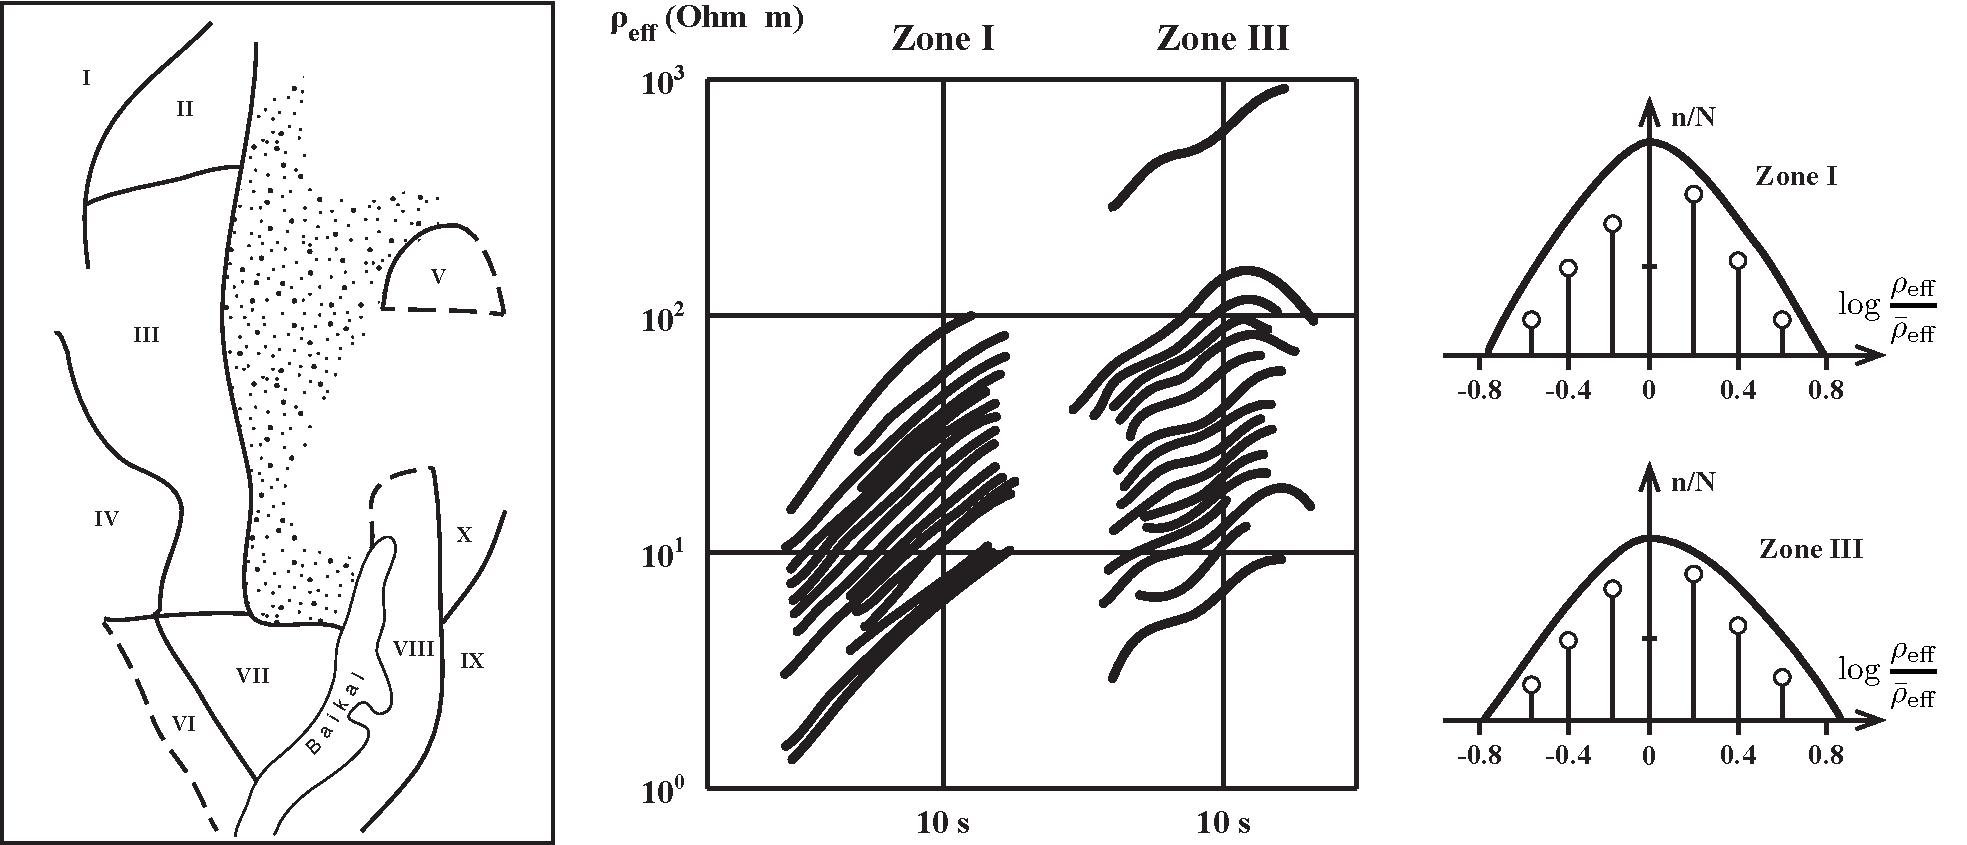
\includegraphics[width=5.5in]{\figdir/berdichevsky_result.pdf}
	\caption[Summary of \citet{berdichevsky1980a}]{(left) Map of Baikal region divided into regions (denoted by numbers), where each has the same conformal effective resistivity curves. (middle) The effective resistivity curves and (right) the distribution of the coefficient $K^i$  from data within Zone I and III \citep[after][]{berdichevsky1980a}.}
	\label{fig:berdichevsky_result}
\end{figure}
	
